\capitulo{6}{Trabajos relacionados}

\section{OpenLaw}

\href{https://www.openlaw.io/}{OpenLaw} es una plataforma que combina contratos inteligentes con protocolos legales convencionales.
Desarrollada para mejorar la eficiencia, seguridad y transparencia en la gestión de acuerdos legales, OpenLaw se posiciona en la vanguardia de la intersección entre la ley y la tecnología blockchain.

La plataforma usa la red Ethereum para registrar cada contrato  en la \textit{blockchain} garantizando que una vez el contrato es firmado, este permanezca inalterable minimizando las posibles disputas sobre el y permitiendo una ejecución automática de los términos acordados.

OpenLaw integra tecnologías de firma digital, facilitando la ratificación de acuerdos sin necesidad de encuentros físicos.
En regiones donde los contratos inteligentes y las firmas digitales están legalmente reconocidos, OpenLaw ofrece una herramienta poderosa y conforme a la ley. Sin embargo, en jurisdicciones sin una regulación clara sobre el uso de la tecnología \textit{blockchain} en el ámbito legal, puede existir incertidumbre sobre la validez y ejecución de estos acuerdos.

En la imagen \ref{img:openLawExample} se puede observar como se ratificaría un contrato usando OpenLaw.

\begin{figure}[h]
	\label{img:openLawExample}
	\centering
	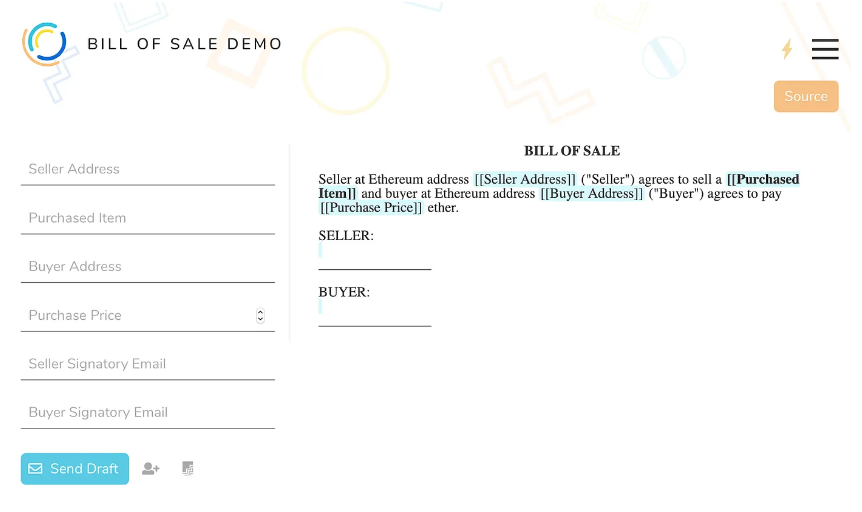
\includegraphics[width=\textwidth]{openLawExample}
	\caption[Ejemplo OpenLaw]{Ejemplo de contrato vinculante usando OpenLaw.}
\end{figure}

\section{Proyectos}

\subsection{TFG - Aplicación web para operar con contratos digitales a través
de blockchain}

El trabajo de Francisco Javier Gozalo Cervera~\cite{tfgSmartContacts} se enfoca en desarrollar una aplicación web destinada a la gestión y operación de contratos digitales utilizando tecnología blockchain.

Su proyecto aborda una necesidad similar al presente trabajo, pero difiere significativamente en su enfoque y ejecución. Gozalo Cervera ha desarrollado una aplicación diseñada específicamente para navegadores web, donde los contratos son creados inicialmente en formato PDF y luego son almacenados en la blockchain para asegurar su integridad y seguridad.

Esta plataforma proporciona una interfaz accesible que permite a los usuarios gestionar sus contratos de manera eficiente y segura, utilizando estándares robustos de tecnología blockchain para garantizar la confiabilidad de los documentos digitales.